\chapter{代数幾何学への導入}\label{ch:ch01}

\begin{chapterlead}
代数幾何学とは，多項式方程式の解全体がなす図形を，多項式のなす環の言葉で調べる学問である．
本章では，以後の章で厳密に展開する理論の「地図」を描くことを目標とする．
まず「図形を方程式で表し，方程式の代数的性質から図形を読み取る」という基本思想を説明し（1.1節），
多項式の零点集合という最も基本的な対象を導入する（1.2節）．
次に実数上と複素数上で零点集合の振る舞いが大きく異なることを見て，複素数上で考えることの利点を確認する（1.3節）．
直線・円錐曲線・楕円曲線・超曲面といった具体例を図とともに眺めたのち（1.4節），
ゲージ理論・超対称理論の真空・弦理論のコンパクト化・Calabi--Yau多様体・モジュライ空間といった物理の話題が，
どのように代数幾何学と結びつくかを概観する（1.5節）．
本章の記述は動機付けを優先しており，厳密な定義と証明は第2章以降で与える．
\end{chapterlead}

%======================================================================
\section{代数幾何学の基本思想}
%======================================================================

\subsection{幾何学的対象と代数的対象}

平面上の単位円を考えよう．これは「原点からの距離が $1$ の点の集合」という幾何学的な記述をもつが，
同時に
\[
  C=\{(x,y)\in\R^2 \mid x^2+y^2-1=0\}
\]
という\textbf{方程式による記述}ももつ．後者の記述では，図形 $C$ は多項式 $f(x,y)=x^2+y^2-1$ という
\emph{代数的な対象}によって完全に決まっている．
代数幾何学の出発点は，この二つの見方を行き来することにある．

もう少し踏み込むと，図形 $C$ 上の「関数」を考えることができる．
$x$ や $y$，$x^2y-3$ のような多項式を $C$ 上に制限したものを $C$ 上の多項式関数と呼ぶ．
$C$ 上では $x^2+y^2=1$ が成り立つので，たとえば $x^2$ と $1-y^2$ は $C$ 上で同じ関数を与える．
したがって $C$ 上の多項式関数全体は，多項式全体を「$x^2+y^2-1$ を $0$ とみなす」という規則で割ったもの，
すなわち剰余環
\[
  \R[x,y]/(x^2+y^2-1)
\]
と同一視される（剰余環の構成は第2章で，この同一視の正当化は第4章・第5章で扱う）．
こうして，図形 $C$ に対して一つの\textbf{環}が対応する．
この環を $C$ の\textbf{座標環}と呼ぶ．

以下の表は，本ノート全体を通じて現れる「幾何と代数の辞書」の一部である．
現時点では右欄の用語の意味がわからなくてもかまわない．各項目は括弧内の章で正確に定式化される．

\begin{table}[H]
\centering
\caption{幾何と代数の辞書（概略）}\label{tab:ch01-dictionary}
\begin{tabular}{ll}
\hline
幾何学的対象 & 代数的対象 \\
\hline
アフィン空間 $\A^n$ & 多項式環 $k[x_1,\dots,x_n]$（第2章，第3章）\\
代数的集合 $X=\Zero(S)$ & 根基イデアル $\Ideal(X)$（第3章，第4章）\\
$X$ 上の多項式関数 & 座標環 $k[X]=k[x_1,\dots,x_n]/\Ideal(X)$（第4章，第5章）\\
$X$ の点 & $k[X]$ の極大イデアル（第4章）\\
既約な図形 & 素イデアル，整域（第3章，第4章）\\
図形の間の写像 & 環準同型（向きが逆）（第5章）\\
点のまわりの様子 & 局所環（第6章）\\
重複した点・「太った点」 & 冪零元をもつ環，スキーム（第12章）\\
\hline
\end{tabular}
\end{table}

この辞書の背後にある原理は，「空間はその上の関数のなす環によって決まる」というものである．
これは代数幾何学に固有の考え方ではなく，たとえば位相空間論における Gelfand--Naimark の定理
（コンパクト Hausdorff 空間は，その上の複素連続関数のなす可換 $C^*$ 環から復元できる）にも現れる．
代数幾何学では，関数として多項式（およびその商）だけを許すことで，この原理が極めて精密かつ計算可能な形で実現される．

\subsection{多項式方程式によって定義される図形}

体 $k$（当面は $k=\R$ または $k=\C$ と思ってよい）と多項式 $f_1,\dots,f_m\in k[x_1,\dots,x_n]$ に対し，
\[
  \{a\in k^n \mid f_1(a)=\dots=f_m(a)=0\}
\]
という形の集合を考える．これが代数幾何学の扱う最も基本的な図形であり，\textbf{代数的集合}と呼ばれる（定義は1.2節，詳しくは第3章）．

代数的集合の例は豊富である．直線 $ax+by+c=0$，円 $x^2+y^2=r^2$，放物線 $y=x^2$，双曲線 $xy=1$，
三次曲線 $y^2=x^3-x$，空間内の球面 $x^2+y^2+z^2=1$，さらに行列の集合
\[
  \SL_2(k)=\{(a,b,c,d)\in k^4\mid ad-bc-1=0\}
\]
もまた代数的集合である．物理に現れる多くの群（$\SL_n$，直交群 $O(n)=\{A\mid A^{\mathsf T}A=I\}$ など）は，
成分に関する多項式方程式で定義されており，代数的集合の構造をもつ．

一方，代数的集合ではない図形も多い．たとえば指数関数のグラフ
\[
  \Gamma=\{(x,y)\in\R^2\mid y=e^x\}
\]
は代数的集合ではない．実際，ある $0$ でない多項式 $f(x,y)=\sum_{i=0}^m a_i(x)y^i$（$a_m\neq0$）が
$\Gamma$ 上で恒等的に $0$ になったとすると，すべての実数 $x$ に対して
$\sum_{i=0}^m a_i(x)e^{ix}=0$ が成り立つ．両辺を $e^{mx}$ で割って $x\to+\infty$ とすると，
$i<m$ の項は $a_i(x)e^{(i-m)x}\to0$ となるので，$a_m(x)\to 0$ でなければならない．
しかし $0$ でない多項式 $a_m(x)$ が $x\to+\infty$ で $0$ に収束することはない（定数なら $0$ でない定数，
次数 $\ge1$ なら発散する）．これは矛盾である．したがって $\Gamma$ を含む代数的集合は $\Gamma$ より真に大きい
（実は $\R^2$ 全体しかない）．
同様に，$y=\sin x$ のグラフも代数的集合ではない（$y=0$ との交わりが無限個の離散点になることから従う．第3章の例\ref{ex:ch03-not-algset}参照）．

このように，代数幾何学は「多項式で書ける図形」に対象を限定する．その代わりに，
多項式環の強力な代数的構造（Noether性，素因数分解，零点定理など）を全面的に使うことができる．

\subsection{幾何学的問題の代数的翻訳}

代数幾何学の威力は，幾何学的な問いを代数的な計算に翻訳できる点にある．簡単な例として，
単位円 $C:\ x^2+y^2=1$ と直線 $L:\ y=mx+c$ の交点を考えよう．
$y=mx+c$ を代入すると
\begin{equation}\label{eq:ch01-circle-line}
  (1+m^2)x^2+2mcx+(c^2-1)=0
\end{equation}
を得る．交点の個数は，この二次方程式の実数解の個数であり，判別式
\[
  D/4=m^2c^2-(1+m^2)(c^2-1)=1+m^2-c^2
\]
の符号で決まる．すなわち
\begin{itemize}
  \item $c^2<1+m^2$ ならば $L$ は $C$ と2点で交わる（割線），
  \item $c^2=1+m^2$ ならば $L$ は $C$ に接する（重解），
  \item $c^2>1+m^2$ ならば $L$ は $C$ と（実数の範囲では）交わらない．
\end{itemize}
「接する」という幾何学的概念が，「方程式が重解をもつ」という代数的条件に翻訳されたことに注意する．
これは後に\textbf{交点の重複度}の概念として一般化される（第9章）．

\begin{figure}[H]
\centering
\begin{tikzpicture}[scale=1.6]
  \draw[->,gray] (-1.8,0)--(1.8,0) node[right]{$x$};
  \draw[->,gray] (0,-1.4)--(0,2.3) node[above]{$y$};
  \draw[thick,blue] (0,0) circle (1);
  \draw[thick,red,domain=-1.8:1.6] plot (\x,{0.5*\x+0.3}) node[right]{割線};
  \draw[thick,red!70!black,dashed,domain=-1.8:1.6] plot (\x,{0.5*\x+1.118}) node[right]{接線};
  \draw[thick,orange,dotted,domain=-1.8:0.6] plot (\x,{0.5*\x+2}) node[right]{交わらない};
  \node[blue] at (0.9,-0.95) {$C$};
\end{tikzpicture}
\caption{単位円と傾き $1/2$ の直線たち．交点の個数は二次方程式 \eqref{eq:ch01-circle-line} の判別式で決まる．}
\label{fig:ch01-circle-line}
\end{figure}

ここで3番目の場合に注目しよう．$c^2>1+m^2$ のとき方程式 \eqref{eq:ch01-circle-line} は実数解をもたないが，
\emph{複素数解}を2つもつ．つまり複素数まで許せば，直線と円は（重複度を込めて）\emph{常に}ちょうど2点で交わる．
さらに，平行な2直線が「無限遠点」で交わると考える射影空間（第8章）まで拡張すると，
「次数 $d$ の曲線と次数 $e$ の曲線は重複度込めてちょうど $de$ 点で交わる」という美しい
\textbf{Bézoutの定理}（第9章）が成り立つ．
実数・アフィン空間での「例外」を取り除くために，複素数と射影空間を用いるのが代数幾何学の基本戦略である．

\subsection{代数的情報から幾何学を復元するという思想}

1.1.1小節で，図形 $X$ に座標環 $k[X]$ が対応することを見た．逆に，環 $k[X]$ から図形 $X$ を復元できるだろうか．
点 $a=(a_1,\dots,a_n)\in X$ に対して，
\[
  \m_a=\{f\in k[X]\mid f(a)=0\}
\]
という $k[X]$ の部分集合を考える．これは「点 $a$ で消える関数全体」であり，$k[X]$ の\textbf{極大イデアル}になる（第2章）．
$k$ が代数閉体（たとえば $k=\C$）のときには，逆に $k[X]$ の極大イデアルはすべてこの形であることが
\textbf{Hilbertの零点定理}（第4章）によって示される．すなわち
\[
  \{X\text{ の点}\}\ \longleftrightarrow\ \{k[X]\text{ の極大イデアル}\}
\]
という一対一対応がある．点という幾何学的概念が，環の中のイデアルという代数的概念によって捉えられたわけである．

さらに Grothendieck は，この思想を徹底して「任意の可換環 $R$ に対して，その素イデアル全体 $\Spec R$ を空間とみなす」
という\textbf{スキーム}の理論を作った（第12章）．そこでは $k[x]/(x^2)$ のように冪零元をもつ環も
「重複した点」として幾何学的に扱われる．

物理学者にとって，この思想は馴染み深いものであろう．量子力学では，状態空間よりも\emph{観測量の代数}が基本的であり，
古典極限では観測量の代数は位相空間上の関数環という可換環になる．
「空間を関数環で置き換える」ことは，非可換幾何学や行列模型の考え方の出発点でもある．

\begin{physbox}[空間と関数環]
古典力学の相空間 $M$ は，その上の関数環 $C^\infty(M)$（観測量の代数）と Poisson 括弧によって特徴付けられる．
量子化はこの可換環を非可換環に変形する操作とみなせる．代数幾何学は，この「関数環が先，空間は後」という見方を
可換環の範囲で徹底したものであり，その非可換版を考える試みが非可換幾何学である．
本ノートでは可換な場合に限るが，第12章のスキーム論や第17章の導来圏の話題において，
この見方の有用性を改めて確認する．
\end{physbox}

本ノート全体の流れを図\ref{fig:ch01-roadmap}にまとめておく．

\begin{figure}[H]
\centering
\begin{tikzpicture}[
  box/.style={draw,rounded corners,align=center,minimum width=3.4cm,minimum height=0.9cm,font=\small},
  >=Stealth]
  \node[box] (I) at (0,0) {第I部 基礎\\ 環論・代数的集合・零点定理};
  \node[box] (II) at (4.6,0) {第II部 アフィン\\ 座標環・局所環・特異点};
  \node[box] (III) at (9.2,0) {第III部 射影\\ 射影空間・Bézout};
  \node[box] (IV) at (2.3,-1.8) {第IV部 大域的構造\\ 有理写像・層・スキーム};
  \node[box] (V) at (6.9,-1.8) {第V部 物理への応用\\ 複素幾何・ゲージ理論・CY・モジュライ};
  \draw[->] (I)--(II); \draw[->] (II)--(III);
  \draw[->] (II)--(IV); \draw[->] (III)--(V); \draw[->] (IV)--(V);
\end{tikzpicture}
\caption{本ノートの構成}\label{fig:ch01-roadmap}
\end{figure}

\exprob{prob:ch01-1-1}
単位円 $x^2+y^2=1$ と放物線 $y=x^2+c$（$c\in\R$）の実数の範囲での交点の個数を，$c$ の値で場合分けして求めよ．
また，複素数の範囲で重複度を込めて数えると，交点の個数は $c$ によらず $4$ であることを確かめよ
（ヒント：$x^2=y-c$ を代入して $y$ の二次方程式を作る）．

\exprob{prob:ch01-1-2}
$y=\log x$（$x>0$）のグラフは $\R^2$ のどの代数的集合とも一致しないことを示せ．

%======================================================================
\section{多項式とその零点集合}
%======================================================================

\subsection{多項式環 $k[x_1,\dots,x_n]$}

$k$ を体とする．変数 $x_1,\dots,x_n$ の\textbf{単項式}とは，多重指数 $\alpha=(\alpha_1,\dots,\alpha_n)\in\N^n$ を用いて
\[
  x^\alpha=x_1^{\alpha_1}x_2^{\alpha_2}\cdots x_n^{\alpha_n}
\]
と書かれるものであり，その\textbf{次数}を $|\alpha|=\alpha_1+\dots+\alpha_n$ と定める．
$k$ 係数の\textbf{多項式}とは，有限個を除いて $0$ であるような係数 $c_\alpha\in k$ を用いた有限和
\[
  f=\sum_{\alpha}c_\alpha x^\alpha
\]
のことである．$c_\alpha\ne0$ となる $\alpha$ に対する $|\alpha|$ の最大値を $f$ の（全）次数と呼び $\deg f$ と書く．
多項式全体は通常の和と積について可換環をなし，これを\textbf{多項式環} $k[x_1,\dots,x_n]$ と書く．
環の一般論は第2章で，多項式環の性質は2.6節で詳しく論じる．

注意すべきは，多項式は本来\emph{形式的な式}であって，関数ではないということである．
各多項式 $f$ は写像 $k^n\to k,\ a\mapsto f(a)$ を定めるが，異なる多項式が同じ写像を定めることがありうる．
たとえば2元体 $k=\F_2=\{0,1\}$ 上では，$x^2-x$ は $0$ でない多項式であるが，$0^2-0=1^2-1=0$ より関数としては恒等的に $0$ である．
しかし $k$ が無限体ならばこのようなことは起こらない．

\begin{myprop}{多項式と多項式関数}{ch01-poly-function}
$k$ を無限体とする．$f\in k[x_1,\dots,x_n]$ がすべての $a\in k^n$ に対して $f(a)=0$ を満たすならば，$f=0$ である．
特に $k$ 上の多項式は，それが定める $k^n$ 上の関数によって一意に決まる．
\end{myprop}

\begin{proof}
$n$ に関する帰納法で示す．$n=1$ のとき，$0$ でない一変数多項式の根の個数は次数以下である（2.6節）から，
無限個の点で消える一変数多項式は $0$ である．
$n\ge2$ とし，$f=\sum_{i=0}^d g_i(x_1,\dots,x_{n-1})x_n^i$ と書く．
任意の $(a_1,\dots,a_{n-1})\in k^{n-1}$ を固定すると，一変数多項式 $\sum_i g_i(a_1,\dots,a_{n-1})x_n^i$ は
$k$ の全ての点で消えるので，$n=1$ の場合より各係数 $g_i(a_1,\dots,a_{n-1})$ は $0$ である．
これが任意の $(a_1,\dots,a_{n-1})$ について成り立つので，帰納法の仮定より $g_i=0$ となり，$f=0$ を得る．
\end{proof}

本ノートで主に扱う $k=\C$（あるいは一般の代数閉体，これは必ず無限体である）では，
多項式と多項式関数を区別する必要はない．
ただし，のちに図形 $X$ 上に制限した関数を考えるときには，「$X$ 上で同じ値をとる多項式」を同一視する必要が生じ，
これが剰余環を考える理由になる．

\begin{myex}{単項式の個数}{ch01-monomial-count}
$n$ 変数の次数 $d$ の単項式の個数は $\binom{n+d-1}{d}$ である．
実際，$x_1^{\alpha_1}\cdots x_n^{\alpha_n}$（$\sum\alpha_i=d$）は，$d$ 個の玉を $n-1$ 本の仕切りで $n$ 組に分ける方法と一対一に対応する．
たとえば $5$ 変数の $5$ 次単項式は $\binom{9}{5}=126$ 個ある．この数は1.5.5小節でQuintic Calabi--Yau多様体の
モジュライを数える際に現れる．
\end{myex}

\subsection{多項式の零点集合}

\begin{mydef}{零点集合}{ch01-zero-set}
$f\in k[x_1,\dots,x_n]$ に対し，
\[
  \Zero(f)=\{a\in k^n\mid f(a)=0\}
\]
を $f$ の\textbf{零点集合}という．$f$ が定数でないとき，$\Zero(f)$ を\textbf{超曲面}と呼ぶ．
$n=2$ のときは\textbf{平面曲線}，$n=3$ のときは\textbf{曲面}とも呼ぶ．
\end{mydef}

ここで $k^n$ を「多項式関数を考える舞台としての空間」とみなしたものを\textbf{アフィン空間}と呼び，$\A^n_k$ あるいは単に $\A^n$ と書く
（第3章）．$\A^n$ は集合としては $k^n$ と同じであるが，原点や線形構造を特別視しない点を強調した記号である．

零点集合の基本的な性質をいくつか挙げておく．
\begin{itemize}
  \item $\Zero(0)=\A^n$，また $c\in k$ が $0$ でない定数ならば $\Zero(c)=\emptyset$．
  \item $\Zero(fg)=\Zero(f)\cup\Zero(g)$．なぜなら体では $f(a)g(a)=0\iff f(a)=0$ または $g(a)=0$ であるから．
  \item $\Zero(f^m)=\Zero(f)$（$m\ge1$）．したがって零点集合からは $f$ の「重複度」の情報が失われる．
\end{itemize}
最後の性質は重要である．$\Zero(x)=\Zero(x^2)$ は $\A^1$ の原点という同じ集合であるが，
$x^2=0$ は「重根」を表すという意味で $x=0$ とは異なる情報をもつ．
この情報を点集合のレベルで捨ててしまうのが古典的な代数幾何学であり（第3章〜第11章），
それを保持するのがスキームの理論である（第12章）．

\begin{myex}{平面曲線}{ch01-plane-curves}
$k=\R$ とする．
(1) $\Zero(x^2+y^2-1)$ は単位円．
(2) $\Zero(xy)=\Zero(x)\cup\Zero(y)$ は2本の座標軸の和集合（図\ref{fig:ch01-zero-sets}左）．
(3) $\Zero(y-x^2)$ は放物線．
(4) $\Zero(y^2-x^3)$ は原点に尖点（cusp）をもつ曲線（1.4.4小節，第7章）．
\end{myex}

\subsection{複数の多項式による共通零点}

一般に，多項式の集合 $S\subset k[x_1,\dots,x_n]$ に対して
\[
  \Zero(S)=\{a\in\A^n\mid \text{すべての }f\in S\text{ に対して }f(a)=0\}=\bigcap_{f\in S}\Zero(f)
\]
と定める．$S=\{f_1,\dots,f_m\}$ が有限集合のときは $\Zero(f_1,\dots,f_m)$ とも書く．
定義から $S\subset T$ ならば $\Zero(S)\supset\Zero(T)$ である（条件が増えれば解は減る）．

$\Zero(S)$ は $S$ そのものよりも，$S$ から「代数的に導かれる」多項式全体によって決まる．
実際，$f,g\in S$ が点 $a$ で消えるならば，任意の多項式 $h_1,h_2$ に対して $h_1f+h_2g$ も $a$ で消える．
そこで $S$ の元の多項式係数の一次結合全体
\[
  (S)=\Big\{\sum_{i=1}^r h_if_i\ \Big|\ r\ge0,\ f_i\in S,\ h_i\in k[x_1,\dots,x_n]\Big\}
\]
を考えると（これを $S$ が生成する\textbf{イデアル}という．第2章），次が成り立つ．

\begin{myprop}{零点集合は生成イデアルのみによる}{ch01-zero-ideal}
$S\subset k[x_1,\dots,x_n]$ に対し，$\Zero(S)=\Zero((S))$ である．
\end{myprop}

\begin{proof}
$S\subset(S)$ より $\Zero(S)\supset\Zero((S))$．逆に $a\in\Zero(S)$ とすると，$(S)$ の任意の元
$\sum h_if_i$ について $\sum h_i(a)f_i(a)=0$ であるから $a\in\Zero((S))$．
\end{proof}

この命題は，連立方程式を「解きやすい形」に変形してよいことの根拠である．たとえば
\[
  \Zero(y-x^2,\ y-1)=\Zero(y-1,\ x^2-1)=\{(1,1),(-1,1)\}
\]
である．ここで $(y-x^2,\,y-1)=(y-1,\,x^2-1)$ は，$x^2-1=(y-1)-(y-x^2)$ と $y-x^2=(y-1)-(x^2-1)$ から従う．
これは連立一次方程式の掃き出し法の非線形版であり，一般には\textbf{Gröbner基底}の理論として体系化されている．

\begin{figure}[H]
\centering
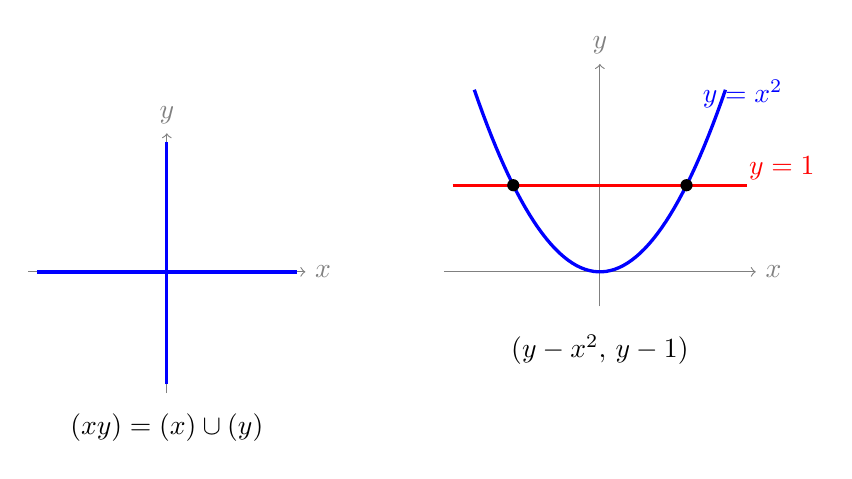
\begin{tikzpicture}[scale=1.1]
  \begin{scope}
    \draw[->,gray] (-1.6,0)--(1.6,0) node[right]{$x$};
    \draw[->,gray] (0,-1.4)--(0,1.6) node[above]{$y$};
    \draw[very thick,blue] (-1.5,0)--(1.5,0);
    \draw[very thick,blue] (0,-1.3)--(0,1.5);
    \node at (0,-1.8) {$\Zero(xy)=\Zero(x)\cup\Zero(y)$};
  \end{scope}
  \begin{scope}[xshift=5cm]
    \draw[->,gray] (-1.8,0)--(1.8,0) node[right]{$x$};
    \draw[->,gray] (0,-0.4)--(0,2.4) node[above]{$y$};
    \draw[very thick,blue,domain=-1.45:1.45,samples=60] plot (\x,{\x*\x});
    \draw[very thick,red] (-1.7,1)--(1.7,1);
    \fill (1,1) circle (2pt) (-1,1) circle (2pt);
    \node[blue] at (1.65,2.05) {$y=x^2$};
    \node[red] at (2.1,1.2) {$y=1$};
    \node at (0,-0.9) {$\Zero(y-x^2,\,y-1)$};
  \end{scope}
\end{tikzpicture}
\caption{和集合と共通部分．積 $xy$ の零点は和集合，連立方程式の零点は共通部分になる．}
\label{fig:ch01-zero-sets}
\end{figure}

\subsection{多項式系によって定義される図形}

$\A^n$ の中で $m$ 個の「独立な」方程式で定まる図形は，直感的には $n-m$ 次元であると期待される．
たとえば $\A^3$ において
\[
  X=\Zero(y-x^2,\ z-x^3)
\]
を考えよう．$X$ の点は $(t,t^2,t^3)$（$t\in k$）と一意にパラメータ表示されるので，$X$ は1次元の曲線である．
これを\textbf{ねじれ三次曲線}（twisted cubic）という．$X$ は2つの曲面 $\Zero(y-x^2)$（放物柱面）と
$\Zero(z-x^3)$ の交わりである．

ところが，「方程式の個数を引けば次元が出る」という素朴な期待はしばしば裏切られる．
\begin{itemize}
  \item $k=\R$ のとき，$\Zero(x^2+y^2)=\{(0,0)\}$ は1個の方程式で定義されるにもかかわらず $0$ 次元である．
        これは実数特有の現象であり，複素数上では $x^2+y^2=(x+iy)(x-iy)$ より $\Zero(x^2+y^2)$ は2直線の和集合（1次元）になる．
  \item $\Zero(x,\ x)=\Zero(x)$ のように，方程式が重複していれば次元は減らない．
  \item より微妙な例として，$\A^3$ の3本の座標軸の和集合 $\Zero(xy,\ yz,\ zx)$ は1次元（余次元2）であるが，
        その定義イデアル $(xy,yz,zx)$ は2個の元では生成できない．このように方程式の個数と余次元が一致しない
        「完全交差でない」例は多数存在する（第7章，第9章）．
\end{itemize}
次元の正確な定義（Krull次元）と，「$m$ 個の方程式で定まる図形の各既約成分の次元は $n-m$ 以上である」という
正しい形の主張は第7章で扱う．
また，代数的集合の全体がある位相（\textbf{Zariski位相}）の閉集合系をなすことを第3章で見る．

\begin{myex}{行列の集合}{ch01-matrices}
$2\times2$ 行列全体を $\A^4$ と同一視する．階数 $\le1$ の行列全体は $\Zero(ad-bc)$ であり，これは $\A^4$ の超曲面（3次元）である．
冪零行列全体は $\Zero(a+d,\ ad-bc)$ であり，「固有多項式 $\lambda^2-(a+d)\lambda+(ad-bc)$ が $\lambda^2$ に等しい」という条件を表す．
これは $\A^4$ の中の2次元の図形（冪零錐）である．
\end{myex}

\exprob{prob:ch01-2-1}
$k=\C$ とし，$\A^2$ において $\Zero(x^2+y^2-1,\ x-y)$ を求めよ．また $\Zero(x^2+y^2-1,\ x^2-y^2)$ を求め，
後者を定義するイデアルが $(x^2-\tfrac12,\ y^2-\tfrac12)$ に等しいことを示せ．

\exprob{prob:ch01-2-2}
$k=\F_p$（$p$ は素数）上で，すべての $a\in k$ に対して $f(a)=0$ を満たす $0$ でない多項式の例を一つ挙げよ
（ヒント：Fermatの小定理）．

%======================================================================
\section{実代数幾何と複素代数幾何}
%======================================================================

\subsection{実数上の代数的集合}

$k=\R$ のとき，代数的集合は我々の直観に最も近い「目に見える」図形である．
しかし同時に，代数的な性質と幾何学的な性質の対応はしばしば崩れる．
典型例は次の3つの曲線である．
\[
  \Zero(x^2+y^2-1),\qquad \Zero(x^2+y^2),\qquad \Zero(x^2+y^2+1).
\]
いずれも「同じ形」の2次方程式で定まるが，実数上ではそれぞれ円・1点・空集合となる（図\ref{fig:ch01-real-circles}）．

\begin{figure}[H]
\centering
\begin{tikzpicture}[scale=0.9]
  \foreach \s/\lab in {0/{$x^2+y^2=1$},4.5/{$x^2+y^2=0$},9/{$x^2+y^2=-1$}}{
    \begin{scope}[xshift=\s cm]
      \draw[->,gray] (-1.6,0)--(1.6,0);
      \draw[->,gray] (0,-1.6)--(0,1.6);
      \node at (0,-2.1) {\lab};
    \end{scope}}
  \draw[very thick,blue] (0,0) circle (1);
  \fill[blue] (4.5,0) circle (2.5pt);
  \node at (9,0.6) {$\emptyset$};
\end{tikzpicture}
\caption{実数上の $x^2+y^2=c$：$c>0$ で円，$c=0$ で1点，$c<0$ で空集合．}
\label{fig:ch01-real-circles}
\end{figure}

実数上の代数的集合には，次のような特有の性質がある．

\begin{myprop}{実数上では1つの方程式で十分}{ch01-real-single}
$f_1,\dots,f_m\in\R[x_1,\dots,x_n]$ に対し，$\R^n$ において
\[
  \Zero(f_1,\dots,f_m)=\Zero(f_1^2+\dots+f_m^2)
\]
が成り立つ．
\end{myprop}

\begin{proof}
実数 $c_1,\dots,c_m$ について，$c_1^2+\dots+c_m^2=0$ と $c_1=\dots=c_m=0$ は同値であることから直ちに従う．
\end{proof}

したがって実数上では「方程式の個数」は幾何学的な意味をもたない．
たとえば $\R^3$ 内の円 $\{x^2+y^2=1,\ z=0\}$ は1つの方程式 $(x^2+y^2-1)^2+z^2=0$ で定義される「超曲面」である．
また，実数上では空でない方程式系と空の方程式系を代数的に区別すること自体が難しい問題であり
（これは Positivstellensatz と呼ばれる実代数幾何学の主題である），本ノートでは深入りしない．

ただし実数上の代数幾何が無意味というわけではない．物理の場面では最終的に実数の量を扱うことが多く，
相空間や配位空間の形状を調べる上で実代数的集合は重要である．本ノートでは，まず複素数上で理論を整え，
実数上の情報は「複素共役で固定される部分」として後から取り出す（1.3.4小節）という立場をとる．

\subsection{複素数上の代数的集合}

$k=\C$ のとき，最も重要な事実は\textbf{代数学の基本定理}である：
定数でない一変数複素係数多項式は必ず $\C$ に根をもつ．
すなわち $\C$ は\textbf{代数閉体}である．これから次元の低い場合について次の主張が得られる．

\begin{myprop}{複素超曲面は空でない}{ch01-complex-nonempty}
$n\ge1$ とし，$f\in\C[x_1,\dots,x_n]$ を定数でない多項式とする．このとき $\Zero(f)\ne\emptyset$ である．
さらに $n\ge2$ ならば $\Zero(f)$ は無限集合である．
\end{myprop}

\begin{proof}
必要なら変数の番号を付け替えて，$f$ は $x_1$ を実際に含むとしてよい．
$f=\sum_{i=0}^dg_i(x_2,\dots,x_n)x_1^i$，$d\ge1$，$g_d\ne0$ と書く．
$n=1$ ならば $g_d$ は $0$ でない定数であり，代数学の基本定理より $f$ は根をもつ．
$n\ge2$ のとき，命題\ref{prop:ch01-poly-function}より $g_d(b_0)\ne0$ となる $b_0\in\C^{n-1}$ が存在する．
さらに，0でないベクトル $e\in\C^{n-1}$ を一つ選ぶと，$t$ の一変数多項式 $g_d(b_0+te)$ は $t=0$ で $0$ でないので
$0$ でない多項式であり，その根は有限個しかない．よって $g_d(b)\ne0$ となる $b$（$=b_0+te$ の形のもの）は無限個存在する．
各そのような $b$ に対して，$f(x_1,b)$ は $x_1$ の $d$ 次多項式であるから根 $a$ をもち，$(a,b)\in\Zero(f)$ となる．
$b$ が異なれば点も異なるので，$\Zero(f)$ は無限集合である．
\end{proof}

この命題は，実数上の $\Zero(x^2+y^2+1)=\emptyset$ のような現象が複素数上では起こらないことを示している．
より一般に，複素数上では「連立方程式系が解をもたないのは，代数的な理由（$1$ が方程式から導かれる）があるときに限る」
という\textbf{弱零点定理}が成り立つ（第4章）．

複素代数的集合を「見る」際には注意が必要である．$\C$ は実2次元であるから，
複素平面曲線 $\Zero(f)\subset\C^2$ は実4次元空間 $\C^2\cong\R^4$ 内の実2次元の曲面である．
たとえば $\Zero(y)\subset\C^2$ は「直線」と呼ばれるが，位相的には平面 $\C\cong\R^2$ である．
したがって複素代数曲線は\textbf{Riemann面}として理解される（第13章）．
本章の図はほとんどが実部分 $\Zero(f)\cap\R^2$ を描いたものであり，これは複素曲線の「一断面」にすぎないことに注意してほしい．

\subsection{実数と複素数における零点の違い}

実数と複素数の違いを，いくつかの観点から比較してみよう．

\paragraph{根の個数．}
一変数 $d$ 次多項式は，複素数上では重複度込めてちょうど $d$ 個の根をもつが，実数上では $0$ 個から $d$ 個まで様々である．
係数を連続的に動かしたとき，実根の個数は不連続に変化しうる（判別式が $0$ を横切るとき，2つの実根が衝突して複素共役な2根になる）．
複素根の個数（重複度込み）は変化しない．
この「数が保存される」という性質は，連続変形のもとで不変な量（交点数，Euler数など）を扱う上で本質的である．

\paragraph{位相の違い：円の複素化．}
複素平面曲線 $C_\C=\{(x,y)\in\C^2\mid x^2+y^2=1\}$ を考える．$u=x+iy$，$v=x-iy$ とおくと
$x^2+y^2=uv$ であるから，
\[
  C_\C\cong\{(u,v)\in\C^2\mid uv=1\}\cong\C^\times=\C\setminus\{0\},\qquad (u,v)\mapsto u
\]
となる（逆写像は $u\mapsto(u,1/u)$）．$\C^\times$ は位相的には円柱 $S^1\times\R$ である
（$u=re^{i\theta}$ に対し $(\theta,\log r)$ を対応させる）．
実部分 $C_\R=C_\C\cap\R^2$ は $v=\bar u$ となる点，すなわち $|u|=1$ の点であり，円柱の「胴回り」の円に相当する
（図\ref{fig:ch01-complex-circle}）．

\begin{figure}[H]
\centering
\begin{tikzpicture}
  \begin{scope}
    \draw[->,gray] (-1.6,0)--(1.6,0) node[right]{$x$};
    \draw[->,gray] (0,-1.6)--(0,1.6) node[above]{$y$};
    \draw[very thick,blue] (0,0) circle (1);
    \node at (0,-2.2) {実部分 $C_\R\cong S^1$};
  \end{scope}
  \begin{scope}[xshift=5.5cm]
    \draw[thick] (-1.2,1.6) ellipse (1.2 and 0.3);
    \draw[thick] (-2.4,1.6)--(-2.4,-1.6);
    \draw[thick] (0,1.6)--(0,-1.6);
    \draw[thick] (-2.4,-1.6) arc (180:360:1.2 and 0.3);
    \draw[thick,dashed,gray] (0,-1.6) arc (0:180:1.2 and 0.3);
    \draw[very thick,blue] (-2.4,0) arc (180:360:1.2 and 0.3);
    \draw[thick,blue,dashed] (0,0) arc (0:180:1.2 and 0.3);
    \node[blue,right] at (0.05,0) {$|u|=1$（実点）};
    \node at (-1.2,2.2) {$|u|\to\infty$};
    \node at (-1.2,-2.25) {$|u|\to0$};
    \node at (-1.2,-2.85) {複素曲線 $C_\C\cong\C^\times$（円柱）};
  \end{scope}
\end{tikzpicture}
\caption{円 $x^2+y^2=1$ の実部分と複素化．複素化は円柱であり，実部分はその胴回りの円である．}
\label{fig:ch01-complex-circle}
\end{figure}

円柱の両端 $|u|\to0$，$|u|\to\infty$ は，射影平面における2つの無限遠点 $[1:\pm i:0]$ に対応する．
これらを付け加えると $C_\C$ は球面 $S^2\cong\PP^1$ になる（第8章，第13章）．
実数上の円がコンパクトであるのに対し複素アフィン曲線は決してコンパクトにならないこと，
そしてコンパクト化するには射影空間が必要であることがこの例からわかる．

\paragraph{双曲線と円．}
実数上では円 $x^2+y^2=1$ と双曲線 $x^2-y^2=1$ は全く異なる形をしている（コンパクトと非コンパクト，連結と非連結）．
しかし複素数上では，座標変換 $y\mapsto iy$ によって両者は同型になる．
実数上の分類（楕円・放物線・双曲線）が複素数上ではより粗い分類に統合されることは，1.4.2小節で再び見る．

\subsection{複素化の意味}

実係数多項式 $f_1,\dots,f_m\in\R[x_1,\dots,x_n]$ に対し，同じ方程式を複素数上で考えた
$X_\C=\Zero(f_1,\dots,f_m)\subset\C^n$ を，実代数的集合 $X_\R=X_\C\cap\R^n$ の\textbf{複素化}という．
$f_i$ の係数は実数なので，複素共役 $\sigma:\C^n\to\C^n$，$\sigma(a)=\bar a$ は $X_\C$ をそれ自身に写す：
\[
  f_i(\bar a)=\overline{f_i(a)}=0.
\]
そして $X_\R$ はちょうど $\sigma$ の固定点集合である．
つまり，\emph{実代数幾何は「複素代数幾何 $+$ 複素共役という対合」}として捉えられる．

複素化の中には，実部分以外にも物理的に意味のある「実の断面」が含まれていることがある．
円 $x^2+y^2=1$ の複素化において，$x\in\R$，$y=i\eta$（$\eta\in\R$）となる点を考えると，
条件は $x^2-\eta^2=1$ となり，これは双曲線である．パラメータで書けば
\[
  (\cos\theta,\ \sin\theta)\ \xrightarrow{\ \theta=i t\ }\ (\cosh t,\ i\sinh t)
\]
であり，回転角 $\theta$ を虚数にする操作が円を双曲線に変える．
これは Euclid 空間の回転群 $SO(2)$ と Lorentz 群 $SO(1,1)$ が，同じ複素群 $SO(2,\C)$ の異なる実形であることの，
最も簡単な現れである．

\begin{physbox}[Wick回転と複素化]
場の量子論における Wick 回転 $t\mapsto -i\tau$ は，Minkowski 計量 $-dt^2+d\vec x^2$ を Euclid 計量 $d\tau^2+d\vec x^2$ に写す．
これは「時間座標を複素化し，複素化された空間の別の実断面を見る」操作に他ならない．
上で見た円と双曲線の関係はその最も簡単な模型である．
一般に，物理量を解析接続して複素領域で考えることで，異なる実断面の間の関係（たとえば Euclid 的な経路積分と
Lorentz 的な時間発展）が見通しよく理解できる．代数幾何学が複素数上で最もよく機能することは，この考え方と相性がよい．
\end{physbox}

\subsection{複素代数幾何が物理に現れる理由}

なぜ理論物理，とりわけ弦理論や超対称ゲージ理論において，\emph{複素}代数幾何がこれほど頻繁に現れるのだろうか．
いくつかの理由を挙げておく．

\begin{enumerate}
  \item \textbf{量子力学は複素数の理論である．}状態ベクトルや確率振幅は複素数値であり，ユニタリ群・複素射影空間
        （純粋状態の空間は $\PP(\mathcal H)$）が自然に現れる．
  \item \textbf{超対称性は正則性をもたらす．}4次元 $\mathcal N=1$ 超対称理論では，超ポテンシャル $W$ はカイラル超場の
        \emph{正則関数}であり，多くの場合多項式である．真空の条件は $\partial W/\partial\phi_i=0$ という多項式方程式になる（1.5.2小節）．
        正則性は非くりこみ定理などの強い制約を生み，厳密な計算を可能にする．
  \item \textbf{2次元の共形対称性は複素構造と結びつく．}弦の世界面は2次元であり，共形構造は Riemann 面の複素構造と同値である
        （第13章）．したがって弦の摂動論は Riemann 面のモジュライ空間上の積分として定式化される．
  \item \textbf{コンパクト化の内部空間は複素多様体である．}超対称性を保つコンパクト化の内部空間として
        Calabi--Yau 多様体が現れ，その多くは射影空間内の多項式方程式で具体的に構成される（1.5.4小節，第15章）．
  \item \textbf{複素数上では数が保存される．}1.3.3小節で見たように，複素数上では解の個数や交点数が変形に対して不変であり，
        これが位相的不変量（指数，Euler数，Gromov--Witten不変量など）と物理量（真空の数，粒子の世代数など）を結びつける．
\end{enumerate}

\begin{physbox}[本ノートにおける複素数の役割]
本ノートでは，第13章以降で複素幾何（複素多様体，Kähler 幾何）と代数幾何の関係を詳しく扱う．
重要な原理は，射影空間内の多項式で定義される図形（射影多様体）は自動的にコンパクト複素多様体になり，
逆に十分よい条件のもとではコンパクト複素多様体が代数的に記述できる（Chowの定理，GAGA）ということである．
これにより，物理で必要な微分幾何学的な量（計量，曲率，ゲージ場）と，代数幾何学的な計算（多項式，次数，交点数）が
結びつけられる．
\end{physbox}

\exprob{prob:ch01-3-1}
$\C^2$ の曲線 $C=\Zero(x^2-y^2-1)$ が $\C^\times$ と全単射に対応することを，具体的な写像を与えて示せ．
また $C\cap\R^2$ はいくつの連結成分をもつか答えよ．

\exprob{prob:ch01-3-2}
実一変数多項式 $f_t(x)=x^3-3x+t$（$t\in\R$）の実根の個数を $t$ の値で分類せよ．
実根の個数が変化する $t$ の値において，$f_t$ は重根をもつことを確かめよ．

%======================================================================
\section{代数幾何学の基本的な例}
%======================================================================

この節では，以後の章で繰り返し登場する基本的な例を図とともに眺める．
各例について (i) 実部分の形，(ii) 複素数上での姿，(iii) 座標環やパラメータ表示といった代数的な記述，の3点に注目する．

\subsection{直線}

平面 $\A^2$ の\textbf{直線}とは，$(a,b)\ne(0,0)$ として一次方程式 $ax+by+c=0$ の零点集合のことである．
直線 $L$ は1点 $p$ と方向ベクトル $v$ を用いて
\[
  \A^1\to L,\qquad t\mapsto p+tv
\]
と全単射にパラメータ表示される．座標環で言えば，たとえば $L=\Zero(y)$ に対して
$k[x,y]/(y)\cong k[x]$ であり，これは「$L$ は $\A^1$ と同型である」ことの代数的な表現である（第5章）．

2本の直線 $L_1:\ a_1x+b_1y=c_1$，$L_2:\ a_2x+b_2y=c_2$ の交わりは，連立一次方程式の解である．
行列式 $a_1b_2-a_2b_1\ne0$ ならばただ1点で交わり，$=0$ ならば平行（交わらないか一致する）である．
「平行な2直線は交わらない」という例外は，射影平面 $\PP^2$ において無限遠直線を付け加えることで解消される：
平行な直線たちは，その方向に対応する無限遠点で交わる（第8章）．

\begin{figure}[H]
\centering
\begin{tikzpicture}[scale=1]
  \begin{scope}
    \draw[->,gray] (-1.8,0)--(1.8,0) node[right]{$x$};
    \draw[->,gray] (0,-1.4)--(0,1.6) node[above]{$y$};
    \draw[very thick,blue] (-1.6,-1.2)--(1.6,1.2);
    \draw[very thick,red] (-1.6,1.0)--(1.6,-0.6);
    \fill (0.457,0.343) circle (2pt);
    \node at (0,-2) {$\det\ne0$：1点で交わる};
  \end{scope}
  \begin{scope}[xshift=5.5cm]
    \draw[->,gray] (-1.8,0)--(1.8,0) node[right]{$x$};
    \draw[->,gray] (0,-1.4)--(0,1.6) node[above]{$y$};
    \draw[very thick,blue] (-1.6,-0.9)--(1.4,1.35);
    \draw[very thick,red] (-1.0,-1.3)--(1.8,0.8);
    \draw[->,dashed,gray] (1.5,1.45)--(2.2,1.97) node[above right]{無限遠点で交わる};
    \node at (0,-2) {$\det=0$：平行};
  \end{scope}
\end{tikzpicture}
\caption{2直線の交わり．平行線は射影平面の無限遠点で交わる．}
\label{fig:ch01-lines}
\end{figure}

一般に，$\A^n$ の\textbf{一次部分多様体}（アフィン部分空間）は連立一次方程式の解集合であり，その次元は線形代数で完全に理解される．
線形代数は「次数1の代数幾何」とみなすことができる．代数幾何学の難しさと面白さは，次数2以上の方程式から生じる．

\subsection{円と二次曲線}

平面の\textbf{二次曲線}（円錐曲線）とは，二次多項式
\[
  f(x,y)=ax^2+bxy+cy^2+dx+ey+g\qquad((a,b,c)\ne(0,0,0))
\]
の零点集合である．実数上では，アフィン変換（平行移動と可逆な一次変換）によって，非退化な二次曲線は
\[
  \text{楕円 } x^2+y^2=1,\qquad \text{放物線 } y=x^2,\qquad \text{双曲線 } x^2-y^2=1
\]
のいずれかに変換できる（ただし $x^2+y^2=-1$ のように実点をもたないものを除く）．
どれになるかは，二次の部分の判別式 $b^2-4ac$ が負・零・正のいずれであるかで決まる．

\begin{figure}[H]
\centering
\begin{tikzpicture}[scale=0.85]
  \begin{scope}
    \draw[->,gray] (-2.2,0)--(2.2,0); \draw[->,gray] (0,-1.6)--(0,1.6);
    \draw[very thick,blue] (0,0) ellipse (1.6 and 1);
    \node at (0,-2.1) {楕円 $b^2-4ac<0$};
  \end{scope}
  \begin{scope}[xshift=5cm,yshift=-1cm]
    \draw[->,gray] (-2.2,0)--(2.2,0); \draw[->,gray] (0,-0.6)--(0,2.6);
    \draw[very thick,blue,domain=-1.55:1.55,samples=60] plot (\x,{\x*\x});
    \node at (0,-1.1) {放物線 $b^2-4ac=0$};
  \end{scope}
  \begin{scope}[xshift=10cm]
    \draw[->,gray] (-2.2,0)--(2.2,0); \draw[->,gray] (0,-1.6)--(0,1.6);
    \draw[very thick,blue,domain=-1.15:1.15,samples=60] plot ({cosh(\x)},{sinh(\x)});
    \draw[very thick,blue,domain=-1.15:1.15,samples=60] plot ({-cosh(\x)},{sinh(\x)});
    \draw[gray,dashed] (-1.6,-1.6)--(1.6,1.6) (-1.6,1.6)--(1.6,-1.6);
    \node at (0,-2.1) {双曲線 $b^2-4ac>0$};
  \end{scope}
\end{tikzpicture}
\caption{実二次曲線の3つの型}
\label{fig:ch01-conics}
\end{figure}

複素数上では，1.3.3小節で見たように楕円と双曲線は区別できなくなり（$y\mapsto iy$），
非退化なアフィン二次曲線は本質的に「$xy=1$ 型」と「$y=x^2$ 型」の2種類になる．
両者の違いは無限遠での振る舞いにある：$xy=1$ 型は無限遠直線と2点で交わり，$y=x^2$ 型は無限遠直線と1点で接する．
射影平面 $\PP^2$ まで考えると，非退化な二次曲線は（複素数上では）すべて互いに射影変換で移りあい，$\PP^1$ と同型になる（第8章）．

\paragraph{円の有理パラメータ表示．}
円 $C:\ x^2+y^2=1$ 上の点 $P=(-1,0)$ を通る傾き $t$ の直線 $y=t(x+1)$ を考える．
これを円の方程式に代入すると $(x+1)\big((1+t^2)x-(1-t^2)\big)=0$ となるので，$P$ 以外の交点は
\begin{equation}\label{eq:ch01-stereo}
  x=\frac{1-t^2}{1+t^2},\qquad y=\frac{2t}{1+t^2}
\end{equation}
である（図\ref{fig:ch01-stereo}）．この直線は $y$ 軸と $(0,t)$ で交わるので，これは $P$ からの\textbf{立体射影}である．
こうして円は，有限個の点を除いて直線と一対一に対応する．このように有理関数でパラメータ表示される曲線を\textbf{有理曲線}という（第10章）．

\begin{figure}[H]
\centering
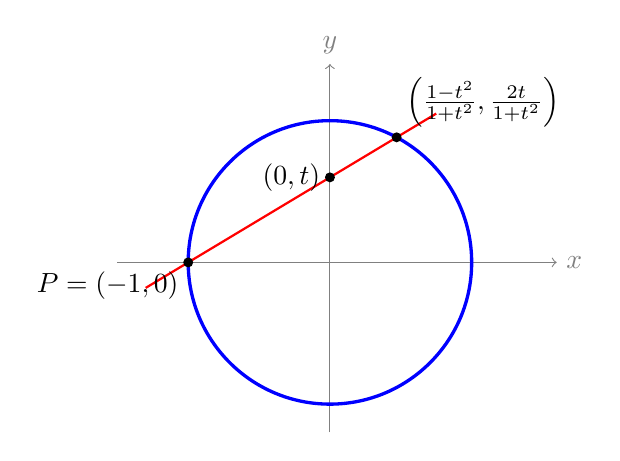
\begin{tikzpicture}[scale=1.8]
  \draw[->,gray] (-1.5,0)--(1.6,0) node[right]{$x$};
  \draw[->,gray] (0,-1.2)--(0,1.4) node[above]{$y$};
  \draw[very thick,blue] (0,0) circle (1);
  \draw[thick,red] (-1.3,-0.18)--(0.75,1.05);
  \fill (-1,0) circle (1pt) node[below left]{$P=(-1,0)$};
  \fill (0,0.6) circle (1pt) node[left]{$(0,t)$};
  \fill (0.4706,0.8824) circle (1pt) node[above right]{$\left(\frac{1-t^2}{1+t^2},\frac{2t}{1+t^2}\right)$};
\end{tikzpicture}
\caption{円の立体射影による有理パラメータ表示}
\label{fig:ch01-stereo}
\end{figure}

式 \eqref{eq:ch01-stereo} は数論的にも興味深い．$t=m/n$ を有理数とすれば $C$ の有理点が得られ，分母を払うと
\[
  (n^2-m^2)^2+(2mn)^2=(n^2+m^2)^2
\]
となって，Pythagoras 数がすべて（定数倍を除いて）得られる．また複素数上では，分母が $0$ になる $t=\pm i$ が
1.3.3小節で見た2つの無限遠点に対応し，$t=\infty$ が点 $P$ に対応する．
したがって複素円 $C_\C$ は $\PP^1$ から2点を除いたもの，すなわち $\C^\times$ と同型であり，1.3.3小節の結果と整合する．

\subsection{放物線}

放物線 $P=\Zero(y-x^2)$ は，多項式 $x^2$ のグラフである．写像
\[
  \A^1\to P,\quad t\mapsto(t,t^2),\qquad P\to\A^1,\quad (x,y)\mapsto x
\]
は互いに逆であり，どちらも多項式で書かれている．したがって $P$ は $\A^1$ と\emph{代数多様体として同型}である（第5章）．
これに対応して，座標環についても
\[
  k[x,y]/(y-x^2)\ \cong\ k[x]
\]
が成り立つ（$y$ を $x^2$ に置き換える写像．2.2.4小節で証明する）．
曲がっている放物線と真っすぐな直線が「同じ」であるというのは奇妙に思えるかもしれないが，
代数幾何学は計量（距離や曲率）ではなく，多項式関数の構造のみを見ているのである．

これと対照的なのが双曲線 $H=\Zero(xy-1)$ である．$H$ の座標環は
\[
  k[x,y]/(xy-1)\ \cong\ k[x,x^{-1}]\qquad(\text{Laurent多項式環})
\]
であり，ここでは $x$ が逆元 $x^{-1}=y$ をもつ．一方，$k[x]$ において逆元をもつのは $0$ でない定数だけである．
環の同型は可逆元を可逆元に写すので，$k[x]\not\cong k[x,x^{-1}]$ であり，したがって $H$ は $\A^1$ と同型ではない．
幾何学的には，$H$ は $x$ 軸への射影によって $\A^1\setminus\{0\}$ と同型であり，「穴が1つ開いた直線」である．
実数上では $H$ は2つの連結成分をもつ（図\ref{fig:ch01-parabola-hyperbola}）が，複素数上では $\C^\times$ は連結である．

\begin{figure}[H]
\centering
\begin{tikzpicture}[scale=0.9]
  \begin{scope}
    \draw[->,gray] (-2,0)--(2,0) node[right]{$x$}; \draw[->,gray] (0,-0.5)--(0,2.6) node[above]{$y$};
    \draw[very thick,blue,domain=-1.55:1.55,samples=60] plot (\x,{\x*\x});
    \draw[thick,->] (0.3,-0.7)--(1.2,-0.7);
    \node at (0,-1.3) {$P=\Zero(y-x^2)\cong\A^1$};
  \end{scope}
  \begin{scope}[xshift=6cm]
    \draw[->,gray] (-2.2,0)--(2.2,0) node[right]{$x$}; \draw[->,gray] (0,-2.2)--(0,2.2) node[above]{$y$};
    \draw[very thick,blue,domain=0.45:2.1,samples=60] plot (\x,{1/\x});
    \draw[very thick,blue,domain=-2.1:-0.45,samples=60] plot (\x,{1/\x});
    \node at (0,-2.7) {$H=\Zero(xy-1)\cong\A^1\setminus\{0\}$};
  \end{scope}
\end{tikzpicture}
\caption{放物線と双曲線．前者は直線と同型，後者は原点を除いた直線と同型である．}
\label{fig:ch01-parabola-hyperbola}
\end{figure}

\begin{myex}{グラフは常にアフィン空間と同型}{ch01-graph}
一般に多項式 $g\in k[x_1,\dots,x_n]$ のグラフ $\Gamma_g=\Zero(x_{n+1}-g(x_1,\dots,x_n))\subset\A^{n+1}$ は，
射影 $(x_1,\dots,x_{n+1})\mapsto(x_1,\dots,x_n)$ によって $\A^n$ と同型である．
座標環では $k[x_1,\dots,x_{n+1}]/(x_{n+1}-g)\cong k[x_1,\dots,x_n]$ に対応する．
\end{myex}

\subsection{楕円曲線}

次数3の平面曲線の中で最も重要なのが\textbf{楕円曲線}である．標数が $2,3$ でない体上では，楕円曲線は
\textbf{Weierstrass形式}
\begin{equation}\label{eq:ch01-weierstrass}
  y^2=x^3+ax+b,\qquad 4a^3+27b^2\ne0
\end{equation}
で表される（正確には，これに射影平面の無限遠点 $O=[0:1:0]$ を1つ付け加えたものである）．
条件 $4a^3+27b^2\ne0$ は，右辺の三次式が重根をもたないことと同値であり，曲線が\textbf{特異点}をもたない（滑らかである）
ことを保証する（第7章）．量 $\Delta=-16(4a^3+27b^2)$ を\textbf{判別式}と呼ぶ．

典型例 $E:\ y^2=x^3-x=x(x-1)(x+1)$ を考えよう（$a=-1,\ b=0$，$4a^3+27b^2=-4\ne0$）．
$y^2\ge0$ でなければならないので，実部分は $x^3-x\ge0$，すなわち $-1\le x\le0$ または $x\ge1$ の範囲にあり，
図\ref{fig:ch01-elliptic}左のように「卵形」と「無限に伸びる枝」の2つの連結成分をもつ．
一般に，$x^3+ax+b$ が相異なる3つの実根をもつとき（$4a^3+27b^2<0$）実部分は2成分，実根が1つのとき（$4a^3+27b^2>0$）1成分である．

\begin{figure}[H]
\centering
\begin{tikzpicture}[scale=0.95]
  \begin{scope}
    \draw[->,gray] (-1.6,0)--(2.5,0) node[right]{$x$}; \draw[->,gray] (0,-3)--(0,3) node[above]{$y$};
    \draw[very thick,blue,domain=0:180,samples=90,smooth]
      plot ({-sin(\x)*sin(\x)},{sin(\x)*cos(\x)*sqrt(1+sin(\x)*sin(\x))});
    \draw[very thick,blue,domain=-1.1:1.1,samples=60,smooth]
      plot ({1+\x*\x},{\x*sqrt((1+\x*\x)*(2+\x*\x))});
    \node at (0.4,-3.5) {$y^2=x^3-x$（滑らか）};
  \end{scope}
  \begin{scope}[xshift=5cm]
    \draw[->,gray] (-1.6,0)--(1.8,0) node[right]{$x$}; \draw[->,gray] (0,-3)--(0,3) node[above]{$y$};
    \draw[very thick,blue,domain=-1.45:1.45,samples=80,smooth]
      plot ({\x*\x-1},{\x*(\x*\x-1)});
    \fill[red] (0,0) circle (2pt);
    \node at (0.1,-3.5) {$y^2=x^2(x+1)$（結節点）};
  \end{scope}
  \begin{scope}[xshift=9.5cm]
    \draw[->,gray] (-0.6,0)--(2,0) node[right]{$x$}; \draw[->,gray] (0,-3)--(0,3) node[above]{$y$};
    \draw[very thick,blue,domain=-1.35:1.35,samples=80,smooth]
      plot ({\x*\x},{\x*\x*\x});
    \fill[red] (0,0) circle (2pt);
    \node at (0.7,-3.5) {$y^2=x^3$（尖点）};
  \end{scope}
\end{tikzpicture}
\caption{楕円曲線 $y^2=x^3-x$ の実部分（左）と，判別式が $0$ になる退化した三次曲線（中・右）．
赤い点は特異点である．}
\label{fig:ch01-elliptic}
\end{figure}

判別式が $0$ になると曲線は特異点をもつ．$y^2=x^2(x+1)$ は原点で自分自身と交わる\textbf{結節点}（node）をもち，
$y^2=x^3$ は原点で尖る\textbf{尖点}（cusp）をもつ（図\ref{fig:ch01-elliptic}）．
これらの特異三次曲線はそれぞれ
\[
  t\mapsto(t^2-1,\ t(t^2-1)),\qquad t\mapsto(t^2,\ t^3)
\]
とパラメータ表示される有理曲線である．
一方，滑らかな楕円曲線は有理関数でパラメータ表示することができない（有理曲線ではない）．

楕円曲線の真価は複素数上で現れる．複素楕円曲線（無限遠点を含む）は，位相的には\textbf{トーラス} $S^1\times S^1$ であり，
複素解析的には格子 $\Lambda=\Z\omega_1+\Z\omega_2\subset\C$ による商 $\C/\Lambda$ と同型である
（Weierstrass の $\wp$ 関数を用いて $(x,y)=(\wp(z),\wp'(z)/2)$ の形で与えられる．定数の規格化は流儀による）．
さらに，楕円曲線上の点には「2点を通る直線と曲線の第3の交点」を用いて\emph{加法}が定義され，アーベル群の構造が入る．
これらの詳細は第13章（Riemann面としての楕円曲線）と第17章（楕円曲線と物理，F理論）で扱う．

\begin{physbox}[楕円曲線と物理]
楕円曲線は，トーラス上の2次元共形場理論（弦の1ループ振幅）において，トーラスの複素構造 $\tau$ として現れる．
また $\mathcal N=2$ 超対称ゲージ理論の低エネルギー有効理論を記述する Seiberg--Witten 曲線（1.5.1小節），
およびF理論において結合定数 $\tau=C_0+ie^{-\phi}$ を幾何学的に表すファイバーとしても現れる（第17章）．
物理において楕円曲線の「形」を変えることは，結合定数などの物理的パラメータを変えることに対応する．
\end{physbox}

\subsection{高次元超曲面}

$\A^n$ の超曲面 $\Zero(f)$ は，1つの方程式で定義される $n-1$ 次元の図形である．
$n=3$ の場合の二次曲面の典型例として，実数 $\varepsilon$ をパラメータとする族
\[
  Q_\varepsilon=\Zero(x^2+y^2-z^2-\varepsilon)\subset\A^3
\]
を考えよう．実数上では，$\varepsilon>0$ のとき一葉双曲面，$\varepsilon=0$ のとき円錐，$\varepsilon<0$ のとき二葉双曲面である
（図\ref{fig:ch01-quadrics}）．

\begin{figure}[H]
\centering
\begin{tikzpicture}[scale=0.75]
  % one-sheeted hyperboloid
  \begin{scope}
    \draw[very thick,blue,domain=-1.2:1.2,samples=50,smooth] plot ({cosh(\x)},{sinh(\x)});
    \draw[very thick,blue,domain=-1.2:1.2,samples=50,smooth] plot ({-cosh(\x)},{sinh(\x)});
    \draw[thick,blue] (0,1.509) ellipse (1.811 and 0.35);
    \draw[thick,blue] (-1.811,-1.509) arc (180:360:1.811 and 0.35);
    \draw[thick,blue,dashed] (1.811,-1.509) arc (0:180:1.811 and 0.35);
    \draw[thick,blue] (-1,0) arc (180:360:1 and 0.2);
    \draw[thick,blue,dashed] (1,0) arc (0:180:1 and 0.2);
    \node at (0,-2.6) {$\varepsilon>0$：一葉双曲面};
  \end{scope}
  % cone
  \begin{scope}[xshift=5.5cm]
    \draw[very thick,blue] (-1.5,1.5)--(1.5,-1.5) (1.5,1.5)--(-1.5,-1.5);
    \draw[thick,blue] (0,1.5) ellipse (1.5 and 0.3);
    \draw[thick,blue] (-1.5,-1.5) arc (180:360:1.5 and 0.3);
    \draw[thick,blue,dashed] (1.5,-1.5) arc (0:180:1.5 and 0.3);
    \fill[red] (0,0) circle (3pt);
    \node at (0,-2.6) {$\varepsilon=0$：円錐（特異点あり）};
  \end{scope}
  % two-sheeted hyperboloid
  \begin{scope}[xshift=11cm]
    \draw[very thick,blue,domain=-1.1:1.1,samples=50,smooth] plot ({sinh(\x)},{cosh(\x)});
    \draw[very thick,blue,domain=-1.1:1.1,samples=50,smooth] plot ({sinh(\x)},{-cosh(\x)});
    \draw[thick,blue] (0,1.669) ellipse (1.336 and 0.3);
    \draw[thick,blue] (-1.336,-1.669) arc (180:360:1.336 and 0.3);
    \draw[thick,blue,dashed] (1.336,-1.669) arc (0:180:1.336 and 0.3);
    \node at (0,-2.6) {$\varepsilon<0$：二葉双曲面};
  \end{scope}
\end{tikzpicture}
\caption{二次曲面の族 $x^2+y^2-z^2=\varepsilon$ の実部分（縦軸が $z$ 軸）．$\varepsilon=0$ で原点に特異点が現れる．}
\label{fig:ch01-quadrics}
\end{figure}

実数上ではこの3つは位相的に全く異なる（連結成分の個数も違う）が，複素数上では $\varepsilon\ne0$ のものはすべて互いに同型であり
（変数を $\sqrt{\varepsilon}$ 倍すればよい），$\varepsilon=0$ のときだけ原点に\textbf{特異点}をもつ円錐が現れる．
すなわち，複素数上では「滑らかな曲面の族が，ある値で特異な曲面に退化する」という描像になる．
これは第7章で扱う特異点の典型例であり，その高次元版（3次元のconifold特異点 $x^2+y^2+z^2+w^2=0$）は
弦理論における幾何学的遷移で中心的な役割を果たす（第17章）．

より一般に，$\PP^n$ の中の $d$ 次超曲面として，\textbf{Fermat超曲面}
\[
  x_0^d+x_1^d+\dots+x_n^d=0
\]
が重要な例を与える．$n=2$，$d=3$ では楕円曲線，$n=3$，$d=4$ では \textbf{K3曲面}，
$n=4$，$d=5$ では\textbf{Quintic三次元多様体}となる．
後二者は「$d=n+1$」という共通の条件を満たしており，これが Calabi--Yau 多様体になるための条件である（1.5.4小節，第15章）．
射影空間内の超曲面の一般論は第9章で扱う．

\exprob{prob:ch01-4-1}
双曲線 $x^2-y^2=1$ 上の点 $(-1,0)$ を通る傾き $t$ の直線を用いて，双曲線の有理パラメータ表示を求めよ．
どの $t$ の値で分母が $0$ になるか，その幾何学的な意味（漸近線との関係）とともに答えよ．

\exprob{prob:ch01-4-2}
$y^2=x^3+ax+b$ について，右辺の三次式 $x^3+ax+b$ が重根をもつことと $4a^3+27b^2=0$ が同値であることを示せ．
（ヒント：重根 $\alpha$ は $\alpha^3+a\alpha+b=0$ かつ $3\alpha^2+a=0$ を満たす．）

%======================================================================
\section{代数幾何学と理論物理}
%======================================================================

この節では，本ノートの第V部（第13章〜第17章）で扱う物理への応用を先取りして概観する．
ここでの説明は直観的なものであり，正確な定義や議論は該当する章で行う．
読者は，ここで出てくる用語の意味がまだわからなくても気にせず，「代数幾何学がどのような場面で必要になるか」をつかんでほしい．

\subsection{ゲージ理論における幾何学}

Maxwell 理論や Yang--Mills 理論といったゲージ理論は，幾何学的には\textbf{主束}上の\textbf{接続}の理論である．
ゲージ場 $A_\mu$ は接続，場の強さ $F_{\mu\nu}$ は曲率，ゲージ変換は束の自己同型に対応する（第14章）．
これだけなら微分幾何学の話であるが，次のような場面で代数幾何学が本質的に現れる．

\begin{itemize}
  \item \textbf{インスタントン．}4次元 Euclid 空間上の反自己双対 Yang--Mills 方程式の解（インスタントン）は，
        ADHM 構成によって，有限次元の行列に関する二次方程式の解を群作用で割ったものとして記述される．
        つまり無限次元の偏微分方程式の解空間が，有限次元の\emph{代数的な}方程式で記述される．
  \item \textbf{正則ベクトル束．}複素曲面上の反自己双対接続は，（適切な条件のもとで）正則ベクトル束と対応する
        （Donaldson--Uhlenbeck--Yau の定理，第14章）．微分方程式の問題が複素代数幾何の問題に翻訳される．
  \item \textbf{Seiberg--Witten理論．}4次元 $\mathcal N=2$ 超対称 $SU(2)$ ゲージ理論の低エネルギー有効理論は，
        パラメータ $u$ をもつ楕円曲線の族（Seiberg--Witten 曲線），たとえばある規格化のもとで
        \[
          y^2=(x^2-u)^2-\Lambda^4
        \]
        によって完全に決定される．ここで $u$ は真空のモジュライ空間の座標であり，楕円曲線が特異になる $u=\pm\Lambda^2$ において
        新たな粒子（モノポールやダイオン）が質量ゼロになる．
\end{itemize}

\subsection{真空の分類と代数的構造}

4次元 $\mathcal N=1$ 超対称理論において，カイラル超場 $\phi_1,\dots,\phi_n$ の超ポテンシャル $W(\phi)$ は正則関数であり，
多くの模型では多項式である．スカラーポテンシャルは $V=\sum_i|\partial W/\partial\phi_i|^2$（ゲージ相互作用がない場合）であり，
超対称な真空（$V=0$）は
\[
  \frac{\partial W}{\partial\phi_1}=\dots=\frac{\partial W}{\partial\phi_n}=0
\]
という\emph{多項式方程式系}の解，すなわち代数的集合である．

\begin{myex}{真空のモジュライの退化}{ch01-vacua}
3つのカイラル超場 $\Phi,X,Y$ と超ポテンシャル $W=\lambda\Phi(XY-\mu^2)$（$\lambda\ne0$）を考える．F項条件は
\[
  \partial_\Phi W=\lambda(XY-\mu^2)=0,\qquad \partial_XW=\lambda\Phi Y=0,\qquad \partial_YW=\lambda\Phi X=0.
\]
$\mu\ne0$ のとき，第1式より $X,Y\ne0$ であるから $\Phi=0$ となり，真空の集合は $\{\Phi=0,\ XY=\mu^2\}\cong\C^\times$ である．
$\mu=0$ のとき，真空の集合は
\[
  \{XY=0,\ \Phi X=0,\ \Phi Y=0\}=\{X=Y=0\}\cup\{\Phi=X=0\}\cup\{\Phi=Y=0\}
\]
となり，原点で交わる3本の直線の和集合になる．パラメータ $\mu$ を $0$ に近づけると，真空の空間は滑らかな曲線から
特異点をもつ図形へと退化し，原点で新たな方向（$\Phi$ 方向）が開く（図\ref{fig:ch01-vacua}）．
\end{myex}

\begin{figure}[H]
\centering
\begin{tikzpicture}[scale=0.9]
  \begin{scope}
    \draw[->,gray] (-2.2,0)--(2.2,0) node[right]{$X$}; \draw[->,gray] (0,-2.2)--(0,2.2) node[above]{$Y$};
    \draw[very thick,blue,domain=0.3:2.1,samples=60] plot (\x,{0.6/\x});
    \draw[very thick,blue,domain=-2.1:-0.3,samples=60] plot (\x,{0.6/\x});
    \node at (0,-2.7) {$\mu\ne0$：$XY=\mu^2$（$\Phi=0$）};
  \end{scope}
  \begin{scope}[xshift=6.5cm]
    \draw[very thick,blue] (-2,0)--(2,0) node[right]{$X$};
    \draw[very thick,blue] (0,-2)--(0,2) node[above]{$Y$};
    \draw[very thick,red] (-1.2,-1.0)--(1.2,1.0) node[above right]{$\Phi$};
    \fill (0,0) circle (2.5pt);
    \node at (0,-2.7) {$\mu=0$：3本の直線};
  \end{scope}
\end{tikzpicture}
\caption{例\ref{ex:ch01-vacua}の真空の集合（実部分の模式図）．}
\label{fig:ch01-vacua}
\end{figure}

ゲージ対称性がある場合には，さらに D 項条件を課してゲージ群で割る必要がある．
多くの場合，この操作は「F項条件の解をゲージ群の複素化 $G_\C$ で割る」という代数的な商と一致し，
真空のモジュライ空間は\emph{ゲージ不変な正則多項式}を座標とする代数多様体として記述される．
たとえば $U(1)$ ゲージ理論で電荷 $\pm1$ のカイラル超場 $Q,\tilde Q$ をもち $W=0$ のとき，
真空のモジュライ空間はゲージ不変量 $M=Q\tilde Q$ を座標とする $\C$ である．
ゲージ不変な多項式が有限個の元で生成されることは Hilbert の不変式論の帰結であり，その背後には第2章で扱う
Hilbert の基底定理がある．真空のモジュライ空間と，それを代数的な商として記述する考え方は第14章（14.6.5小節）と第16章で触れる．

\subsection{弦理論におけるコンパクト化}

超弦理論は10次元時空で整合的に定義される．我々の観測する4次元時空を得るには，残りの6次元を小さなコンパクト空間 $K$ に
巻き上げる必要がある：
\[
  M_{10}=M_4\times K_6.
\]
これを\textbf{コンパクト化}という．最も簡単な例として，5次元の質量ゼロのスカラー場を半径 $R$ の円 $S^1$ 上にコンパクト化すると，
円方向の運動量が量子化され，4次元では質量 $|n|/R$（$n\in\Z$）の粒子の無限個の塔（Kaluza--Klein モード）が現れる．
$R$ が小さければ $n\ne0$ のモードは重く，低エネルギーでは $n=0$ のモードだけが残る．

一般に，4次元の低エネルギー有効理論の粒子の種類や相互作用は，内部空間 $K$ の幾何学的・位相的性質
（Betti数，交点数，ベクトル束の Chern 類など）によって決まる．
たとえば，ヘテロティック弦理論の Calabi--Yau コンパクト化では，フェルミオンの世代数が $K$ の Euler 数の半分の絶対値 $|\chi(K)|/2$
で与えられるという古典的な結果がある（標準埋め込みの場合）．
このように，\emph{物理的な量が幾何学的な不変量として計算される}ことがコンパクト化の要点であり，
その不変量を計算する道具として代数幾何学が用いられる（第15章）．

\subsection{Calabi--Yau多様体}

4次元で $\mathcal N=1$ 超対称性を保つコンパクト化の条件を調べると，内部空間 $K$ は
（フラックスなどがない最も簡単な状況で）\textbf{Calabi--Yau 3次元多様体}であることが要請される
（Candelas--Horowitz--Strominger--Witten，1985年）．
Calabi--Yau 多様体の大まかな定義は「コンパクトな Kähler 多様体で，第一 Chern 類が消えるもの」であり，
Calabi 予想（Yau により証明）によって，このとき Ricci 平坦な Kähler 計量が存在する．

\begin{note}
Calabi--Yau 多様体の定義は文献によって異なる．標準束が自明であること，第一Chern類（実係数）が $0$ であること，
ホロノミー群が $SU(n)$ に含まれる（あるいは一致する）こと，$h^{p,0}=0$（$0<p<n$）を課すかどうか，などの流儀がある．
単連結性などの条件のもとでこれらは同値になるが，一般には一致しない．詳しくは第15章で論じる．
\end{note}

代数幾何学の立場から重要なのは，Calabi--Yau 多様体の多くが\emph{射影空間内の多項式方程式によって具体的に構成できる}ことである．
$\PP^n$ の滑らかな $d$ 次超曲面が（標準束が自明という意味で）Calabi--Yau になる条件は $d=n+1$ である（第15章）．
したがって
\begin{itemize}
  \item 1次元：$\PP^2$ の三次曲線（楕円曲線），
  \item 2次元：$\PP^3$ の四次曲面（K3曲面），
  \item 3次元：$\PP^4$ の五次超曲面（Quintic），たとえば $x_0^5+x_1^5+x_2^5+x_3^5+x_4^5=0$
\end{itemize}
が Calabi--Yau 多様体の基本例となる．Quintic の Hodge 数は $h^{1,1}=1$，$h^{2,1}=101$ であり，Euler 数は
$\chi=2(h^{1,1}-h^{2,1})=-200$ である．
重み付き射影空間内の超曲面や完全交差を用いると，さらに多くの例が得られる（第15章）．

\subsection{モジュライ空間と物理的自由度}

Calabi--Yau 多様体は1つではなく，連続的なパラメータをもつ族として存在する．
「ある種類の幾何学的対象の同型類全体」がなす空間を\textbf{モジュライ空間}と呼ぶ（第16章）．

最も簡単な例は楕円曲線である．Weierstrass 形式 \eqref{eq:ch01-weierstrass} の楕円曲線 $y^2=x^3+ax+b$ の同型類は，
\textbf{$j$不変量}
\[
  j=1728\,\frac{4a^3}{4a^3+27b^2}
\]
によって完全に分類される（代数閉体上）．すなわち，$(a,b)$ という2つのパラメータのうち，同型で移りあう分（$(a,b)\mapsto(\lambda^4a,\lambda^6b)$）
を除いた1次元の自由度 $j$ が楕円曲線の「形」を表し，楕円曲線のモジュライ空間は $j$ 直線 $\A^1$ である．
複素解析的には，これはトーラス $\C/(\Z+\Z\tau)$ の複素構造 $\tau$ を $\SL(2,\Z)$ で割ったものに対応する（第13章，第17章）．

Quintic Calabi--Yau の場合にも同様の勘定ができる．5変数の5次単項式は $126$ 個あるから（例\ref{ex:ch01-monomial-count}），
5次多項式の係数は126個のパラメータをもつ．このうち $\GL_5(\C)$ による座標変換（次元25）で移りあうものは同型であるから，
本質的なパラメータの数は
\[
  126-25=101
\]
であり，これはちょうど Hodge 数 $h^{2,1}=101$ に一致する．これが Quintic の\textbf{複素構造モジュライ}の次元である．
同様の勘定で，$\PP^2$ の三次曲線は $\binom{5}{2}-9=10-9=1$，$\PP^3$ の四次曲面は $\binom{7}{3}-16=35-16=19$ 個の
パラメータをもつ．

\begin{physbox}[モジュライ場]
コンパクト化において，内部空間 $K$ の形や大きさを表すモジュライは，4次元時空の各点で値をとる場，すなわち\textbf{モジュライ場}となる．
モジュライの方向にはポテンシャルが（摂動論的には）生じないので，モジュライ場は4次元で質量ゼロのスカラー場として現れる．
Quintic の場合，101個の複素構造モジュライと1個の Kähler モジュライ（大きさ）が，それぞれ4次元のスカラー場の自由度を与える．
観測とのつじつまを合わせるにはこれらの場に質量を与える機構（モジュライ安定化）が必要であり，これは現代の弦理論の重要な課題である．
複素構造モジュライと Kähler モジュライを入れ替える双対性がミラー対称性であり（第17章），
モジュライ空間の幾何学そのものが物理の重要な研究対象となっている．詳細は第16章で扱う．
\end{physbox}

\exprob{prob:ch01-5-1}
$y^2=x^3+ax+b$ において $(a,b)\mapsto(\lambda^4a,\lambda^6b)$（$\lambda\ne0$）としても $j$ 不変量が変わらないことを確かめよ．
また，この変換が座標変換 $(x,y)\mapsto(\lambda^2x,\lambda^3y)$ から生じることを示せ．

\exprob{prob:ch01-5-2}
$\PP^n$ の $d$ 次超曲面の定義多項式の係数の個数から $\GL_{n+1}$ の次元を引いた数 $\binom{n+d}{d}-(n+1)^2$ を，
$(n,d)=(2,3),(3,4),(4,5)$ について計算し，本文の値と一致することを確かめよ．

\section*{問題の解答}
\addcontentsline{toc}{section}{問題の解答}

\exsol{prob:ch01-1-1}
$y=x^2+c$ を $x^2+y^2=1$ に代入すると，$x$ の四次方程式
\[
  x^4+(2c+1)x^2+(c^2-1)=0
\]
を得る．逆にこの解 $x$ に対して $y=x^2+c$ と定めれば交点が得られ，交点と解 $x$ は一対一に対応する．
ヒントに従って $x^2=y-c$ を円の式に代入すると
\[
  g(y):=y^2+y-(1+c)=0
\]
となる．各交点の $y$ 座標は $g(y)=0$ の根であり，逆に根 $y$ に対して $x^2=y-c$ を満たす $x$ をとれば交点が得られる．
したがって実の交点を数えるには，$g$ の実根 $y$ のうち $y\ge c$ を満たすものを調べればよい
（$y>c$ なら $x=\pm\sqrt{y-c}$ の2点，$y=c$ なら $x=0$ の1点が対応する）．

$g$ の判別式は $1+4(1+c)=4c+5$ であり，実根は $y_\pm=\dfrac{-1\pm\sqrt{4c+5}}{2}$，$y_-\le-\tfrac12\le y_+$ である．
また $g(c)=c^2-1$ である．$g$ は下に凸なので，$c$ が2根の間にあるのは $g(c)<0$ のとき，2根より小さいのは $g(c)>0$ かつ $c<-\frac12$ のとき，
2根より大きいのは $g(c)>0$ かつ $c>-\frac12$ のときである．これより次のように場合分けされる．
\begin{itemize}
  \item $c<-\frac54$：実根がないので交点は $0$ 個．
  \item $c=-\frac54$：重根 $y=-\frac12$ で $y-c=\frac34>0$．交点は $(\pm\frac{\sqrt3}2,-\frac12)$ の $2$ 個（それぞれで接する）．
  \item $-\frac54<c<-1$：$g(c)>0$，$c<-\frac12$ なので $c<y_-<y_+$．交点は $4$ 個．
  \item $c=-1$：$g(y)=y(y+1)$ で根は $-1=c$ と $0$．交点は $(0,-1)$ と $(\pm1,0)$ の $3$ 個．
  \item $-1<c<1$：$g(c)<0$ なので $y_-<c<y_+$．$y_+$ のみが寄与し，交点は $2$ 個．
  \item $c=1$：$g(y)=(y-1)(y+2)$ で $y_+=1=c$．交点は $(0,1)$ の $1$ 個．
  \item $c>1$：$g(c)>0$，$c>-\frac12$ なので $y_-<y_+<c$．交点は $0$ 個．
\end{itemize}

複素数の範囲では，上の $x$ の四次方程式は最高次係数が $1$ なので，代数学の基本定理により重複度を込めてちょうど $4$ 個の根をもち，
各根 $x$ に交点 $(x,x^2+c)$ がただ一つ対応する．よって交点は重複度込みで $c$ によらず $4$ 個である．
ヒントの方法で言えば，$g(y)=0$ が重複度込みで $2$ 根をもち，各根 $y$ に対して $x^2=y-c$ が重複度込みで $2$ 根をもつので $2\times2=4$ である．
たとえば $c=-1$ では $x^4-x^2=x^2(x-1)(x+1)$ で $x=0$ が二重根（点 $(0,-1)$ で接する），
$c=1$ では $x^4+3x^2=x^2(x^2+3)$ で $x=0$ が二重根，残り2個は虚の交点 $(\pm\sqrt3\,i,-2)$，
$c=-\frac54$ では $x^4-\frac32x^2+\frac9{16}=(x^2-\frac34)^2$ で2点がそれぞれ二重に数えられる．

\exsol{prob:ch01-1-2}
グラフ $\Gamma=\{(x,\log x)\mid x>0\}$ が代数的集合 $\Zero(f_1,\dots,f_m)$（$f_i\in\R[x,y]$）に等しいと仮定する．
$F=f_1^2+\dots+f_m^2$ とおくと，実数の範囲では $F(P)=0\iff f_1(P)=\dots=f_m(P)=0$ なので $\Gamma=\Zero(F)$ である．
$\Gamma\ne\R^2$ だから $F\ne0$ である．

$F=\sum_{i,j}a_{ij}x^iy^j$ と書き，$x=e^t$（$t\in\R$）を代入すると，すべての $t\in\R$ に対して
\[
  0=F(e^t,t)=\sum_{i=0}^{N}b_i(t)\,e^{it},\qquad b_i(t)=\sum_ja_{ij}t^j\in\R[t]
\]
が成り立つ．$F\ne0$ なので $b_i\ne0$ となる $i$ があり，そのような $i$ の最大値を改めて $N$ とする．両辺を $e^{Nt}$ で割ると
\[
  b_N(t)=-\sum_{i=0}^{N-1}b_i(t)\,e^{-(N-i)t}.
\]
$t\to+\infty$ のとき，右辺の各項は（多項式）$\times$（指数関数的に減少する関数）なので $0$ に収束する．
一方，$0$ でない多項式 $b_N(t)$ は $t\to+\infty$ で $0$ に収束しない（定数なら $0$ でない定数，次数 $1$ 以上なら $\pm\infty$ に発散する）．
これは矛盾である．よって $\Gamma$ はどの代数的集合とも一致しない．
本質は，$\log x$（あるいは $e^t$）が多項式の関係式を満たさない，すなわち超越的な関数であることにある．

\exsol{prob:ch01-2-1}
$\Zero(x^2+y^2-1,\ x-y)$：$y=x$ を代入して $2x^2=1$，$x=\pm\frac1{\sqrt2}$．よって
\[
  \Zero(x^2+y^2-1,\ x-y)=\Bigl\{\bigl(\tfrac1{\sqrt2},\tfrac1{\sqrt2}\bigr),\ \bigl(-\tfrac1{\sqrt2},-\tfrac1{\sqrt2}\bigr)\Bigr\}.
\]
$\Zero(x^2+y^2-1,\ x^2-y^2)$：$f=x^2+y^2-1$，$g=x^2-y^2$ とおくと
\[
  x^2-\tfrac12=\tfrac12(f+g),\qquad y^2-\tfrac12=\tfrac12(f-g),\qquad
  f=\bigl(x^2-\tfrac12\bigr)+\bigl(y^2-\tfrac12\bigr),\qquad g=\bigl(x^2-\tfrac12\bigr)-\bigl(y^2-\tfrac12\bigr).
\]
前の2式から $x^2-\frac12,\ y^2-\frac12$ は $f,g$ の多項式係数の一次結合であり，後の2式からその逆も成り立つ．
したがって $f,g$ の生成するイデアルと $x^2-\frac12,\ y^2-\frac12$ の生成するイデアルは等しい：
\[
  (x^2+y^2-1,\ x^2-y^2)=\bigl(x^2-\tfrac12,\ y^2-\tfrac12\bigr).
\]
零点集合はイデアルのみで決まるので
\[
  \Zero(x^2+y^2-1,\ x^2-y^2)=\Zero\bigl(x^2-\tfrac12,\ y^2-\tfrac12\bigr)=\Bigl\{\bigl(\pm\tfrac1{\sqrt2},\ \pm\tfrac1{\sqrt2}\bigr)\Bigr\}
\]
（複号任意の4点）である．幾何学的には，$x^2-y^2=(x-y)(x+y)$ なので，これは円と二直線 $y=\pm x$ の交点である．

\exsol{prob:ch01-2-2}
$f=x^p-x\in\F_p[x]$ とすればよい．$f$ は次数 $p$ の多項式なので零多項式ではない．
一方 Fermat の小定理により，すべての $a\in\F_p$ について $a^p=a$（$a=0$ では自明，$a\ne0$ では $a^{p-1}=1$）だから $f(a)=0$ である．
実際 $x^p-x=\prod_{a\in\F_p}(x-a)$ であり，$\F_p$ のすべての元を根にもつ．
これは，有限体上では「多項式」と「多項式関数」を区別しなければならないことを示している．

\exsol{prob:ch01-3-1}
$x^2-y^2=(x+y)(x-y)$ なので，$C$ は $(x+y)(x-y)=1$ で定まる．写像
\[
  \Phi\colon C\to\C^\times,\quad (x,y)\mapsto u=x+y,\qquad
  \Psi\colon\C^\times\to C,\quad u\mapsto\Bigl(\frac{u+u^{-1}}2,\ \frac{u-u^{-1}}2\Bigr)
\]
を考える．$(x,y)\in C$ なら $(x+y)(x-y)=1$ より $u=x+y\ne0$ なので $\Phi$ は well-defined である．
また $\Psi(u)$ について $x+y=u$，$x-y=u^{-1}$ なので $x^2-y^2=u\cdot u^{-1}=1$，すなわち $\Psi(u)\in C$．
$\Phi\circ\Psi(u)=u$ は明らか．逆に $(x,y)\in C$ に対し $x-y=(x+y)^{-1}=u^{-1}$ なので
$x=\frac{u+u^{-1}}2$，$y=\frac{u-u^{-1}}2$，すなわち $\Psi\circ\Phi=\mathrm{id}_C$．よって $\Phi$ は全単射である．
（本文の双曲線 $xy=1$ の場合と同じく，$C$ は $\C^\times$ と同型であり，複素数上では連結である．）

$C\cap\R^2$ は実双曲線 $x^2-y^2=1$ である．$x^2=1+y^2\ge1$ より $x\ge1$ または $x\le-1$ であり，
それぞれの部分は $y\mapsto(\pm\sqrt{1+y^2},y)$ によって $\R$ と同相なので連結である．一方 $\{x\ge1\}$ と $\{x\le-1\}$ は直線 $x=0$ で分離される．
よって $C\cap\R^2$ の連結成分は $2$ 個である．上の対応では，実の点は $u\in\R^\times$ に対応し，$\R^\times=\R_{>0}\sqcup\R_{<0}$ の2成分がそのまま2本の枝になる．

\exsol{prob:ch01-3-2}
$f_t'(x)=3x^2-3=3(x-1)(x+1)$ なので，$f_t$ は $x=-1$ で極大値 $f_t(-1)=t+2$，$x=1$ で極小値 $f_t(1)=t-2$ をとり，
$x\to\pm\infty$ で $f_t(x)\to\pm\infty$ である．中間値の定理と増減から
\begin{itemize}
  \item $|t|<2$（極大値 $>0$，極小値 $<0$）：相異なる実根が $3$ 個，
  \item $|t|=2$：相異なる実根が $2$ 個（うち1つは重根），
  \item $|t|>2$（極大値と極小値が同符号）：実根は $1$ 個
\end{itemize}
となる．実根の個数が変化するのは $t=\pm2$ であり，このとき
\[
  f_2(x)=x^3-3x+2=(x-1)^2(x+2),\qquad f_{-2}(x)=x^3-3x-2=(x+1)^2(x-2)
\]
となって，確かに重根 $x=1$，$x=-1$ をもつ．三次式 $x^3+px+q$ の判別式 $-4p^3-27q^2$ を用いれば，
$-4(-3)^3-27t^2=27(4-t^2)$ が $0$ になる $t$ がちょうど $\pm2$ であることからも確かめられる．
重根は二つの実根が合流して（$|t|>2$ 側では）一組の共役な虚根に変わる瞬間を表している．

\exsol{prob:ch01-4-1}
点 $(-1,0)$ を通る傾き $t$ の直線 $y=t(x+1)$ を $x^2-y^2=1$ に代入すると
\[
  x^2-1-t^2(x+1)^2=(x+1)\bigl[(x-1)-t^2(x+1)\bigr]=0.
\]
因子 $x+1$ は既知の交点 $(-1,0)$ に対応し，もう一つの交点は $(1-t^2)x=1+t^2$ から得られる：
\[
  x=\frac{1+t^2}{1-t^2},\qquad y=t(x+1)=\frac{2t}{1-t^2}.
\]
実際 $(1+t^2)^2-(2t)^2=(1-t^2)^2$ なので $x^2-y^2=1$ を満たす．
逆に双曲線上の点 $(x,y)\ne(-1,0)$ では $x\ne-1$（$x=-1$ なら $y=0$）なので $t=y/(x+1)$ が定まり，上の式で表される．
（点 $(-1,0)$ 自身は，そこでの接線である垂直線 $x=-1$，すなわち $t=\infty$ に対応する．）

分母が $0$ になるのは $t=\pm1$ のときである．このとき直線 $y=\pm(x+1)$ は双曲線の漸近線 $y=\pm x$ と平行であり，
上の式で $(1-t^2)x=1+t^2$ が $0=2$ となって解をもたない．すなわち2番目の交点が存在せず，「無限遠に逃げた」と解釈できる．
射影平面（第8章以降）で考えると，これは漸近線方向の無限遠点 $[1:\pm1:0]$ が双曲線上にあり，$t=\pm1$ がそれらに対応していることを意味する．

\exsol{prob:ch01-4-2}
$f(x)=x^3+ax+b$ とする（係数体は標数 $2,3$ でない体，たとえば $\C$ とする）．
まず，$\alpha$ が $f$ の重根であることと $f(\alpha)=f'(\alpha)=0$ が同値であることに注意する．
実際 $f=(x-\alpha)^2g$ なら $f'=2(x-\alpha)g+(x-\alpha)^2g'$ より $f'(\alpha)=0$．
逆に $f(\alpha)=0$ なら $f=(x-\alpha)h$ と書けて $f'=h+(x-\alpha)h'$ なので，$f'(\alpha)=0$ なら $h(\alpha)=0$，すなわち $(x-\alpha)^2\mid f$．
したがって重根 $\alpha$ は
\[
  \alpha^3+a\alpha+b=0,\qquad 3\alpha^2+a=0
\]
を満たす $\alpha$ に他ならない（$\C$ で考えれば根は必ず存在する）．

\textbf{$a=0$ の場合．}第2式から $\alpha=0$，第1式から $b=0$．逆に $a=b=0$ なら $f=x^3$ は重根をもつ．
よって重根をもつ $\iff b=0\iff4a^3+27b^2=0$．

\textbf{$a\ne0$ の場合．}重根 $\alpha$ があるとする．第2式より $\alpha^2=-\frac a3$ なので第1式は
$\alpha(\alpha^2+a)+b=\frac{2a}3\alpha+b=0$，すなわち $\alpha=-\dfrac{3b}{2a}$．これを第2式に代入して
\[
  3\cdot\frac{9b^2}{4a^2}+a=\frac{27b^2+4a^3}{4a^2}=0,
\]
よって $4a^3+27b^2=0$．逆に $4a^3+27b^2=0$ のとき $\alpha=-\frac{3b}{2a}$ とおけば，上の計算から $3\alpha^2+a=0$ であり，
\[
  \alpha^3+a\alpha+b=\alpha(\alpha^2+a)+b=\alpha\cdot\frac{2a}3+b=-b+b=0
\]
となるので，$\alpha$ は重根である．以上で同値性が示された．

\exsol{prob:ch01-5-1}
$a'=\lambda^4a$，$b'=\lambda^6b$ とおくと
\[
  4a'^3+27b'^2=\lambda^{12}(4a^3+27b^2),\qquad
  j(a',b')=1728\,\frac{4\lambda^{12}a^3}{\lambda^{12}(4a^3+27b^2)}=1728\,\frac{4a^3}{4a^3+27b^2}=j(a,b)
\]
であり，$j$ は変わらない（$4a^3+27b^2\ne0$ も保たれる）．

次に $(X,Y)=(\lambda^2x,\lambda^3y)$ とおく．$(x,y)$ が $y^2=x^3+ax+b$ を満たすならば
\[
  Y^2=\lambda^6y^2=\lambda^6x^3+\lambda^6ax+\lambda^6b=X^3+(\lambda^4a)X+\lambda^6b
\]
となり，$(X,Y)$ は $Y^2=X^3+a'X+b'$ を満たす．逆変換 $(x,y)=(\lambda^{-2}X,\lambda^{-3}Y)$ も同じ形なので，
この座標変換は曲線 $y^2=x^3+ax+b$ と $y^2=x^3+a'x+b'$ の間の全単射（どちらの向きも多項式で書ける同型）を与える．
したがってパラメータの変換 $(a,b)\mapsto(\lambda^4a,\lambda^6b)$ は座標変換 $(x,y)\mapsto(\lambda^2x,\lambda^3y)$ から生じている．
この変換で $x$ は重さ $2$，$y$ は重さ $3$，$a$ は重さ $4$，$b$ は重さ $6$ をもち，$a^3$ と $b^2$ がともに重さ $12$ なので，
その比である $j$ が不変量になる．

\exsol{prob:ch01-5-2}
$n+1$ 変数の $d$ 次単項式の個数は $\binom{n+d}{d}$，$\dim\GL_{n+1}=(n+1)^2$ である．
\begin{itemize}
  \item $(n,d)=(2,3)$：$\binom{5}{3}-3^2=10-9=1$．
  \item $(n,d)=(3,4)$：$\binom{7}{4}-4^2=35-16=19$．
  \item $(n,d)=(4,5)$：$\binom{9}{5}-5^2=126-25=101$．
\end{itemize}
本文の値（三次曲線 $1$，四次曲面 $19$，Quintic $101$）と一致する（$\binom52=\binom53$，$\binom73=\binom74$ に注意）．
三次曲線の $1$ は楕円曲線の $j$ 不変量の1次元に，四次曲面（K3曲面）の $19$ は代数的 K3 曲面の複素構造モジュライの次元に，
$101$ は Quintic の $h^{2,1}$ に対応している．

なお，超曲面は定義多項式の定数倍によらないので，正確には「係数の空間 $\binom{n+d}{d}$ 次元から定数倍の $1$ を引き，
$\mathrm{PGL}_{n+1}$（次元 $(n+1)^2-1$）で割る」と数えるべきであるが，
$\bigl(\binom{n+d}{d}-1\bigr)-\bigl((n+1)^2-1\bigr)=\binom{n+d}{d}-(n+1)^2$ なので結果は同じである
（$\GL_{n+1}$ のスカラー行列が多項式を定数倍することに対応する）．
